%%%%%%%%%%%%%%%%%%%%%%%%%%%%%%%%%%%%%%%%%%%%%%%%%%%%%%%%%%%%%%%%%%%%%%%%%%%%%%%%%

\hypertarget{appendix:a}{} %% uso para este Guia
\renewcommand{\thechapter}{}%
\chapter{APPENDIX A - INTERSECTION ALGORITHMS}
\label{ap:a}
\renewcommand{\thechapter}{A}

\section{Problem}\label{ap:a:problem}

This is only a simple overview to show the importance of the problem and how different algorithms stack against each other.

The problem can be stated as follows: given sets $S_1$ and $S_2$, find the elements that are present in both sets, their intersection, represented as $S_1 \cap S_2$.
Furthermore, each element is ordered and unique (non-repeating), as they represented index positions and are thus always non-zero positive integers.

\section{Algorithms}\label{ap:a:algos}

This section details the compared algorithms, giving more information on the ones that deviate from literature further.

The UnorderedSet algorithm is an implementation of the optimum complexity algorithm: iterate over all elements of one vector and use a hashing function to check for equality, adding the elements that are equal.
This is an $\mathcal{O}(n+m)$ operation, with $n$ and $m$ the size of both lists.
For this work, the UnorderedSet functions from the C++ standard were used for brevity.

The Scalar algorithm, also called the naïve or the tape-merge algorithm, is the standard way of computing the intersection between two lists \cite{hwangSimpleAlgorithmMerging1972}.
It is detailed in Algorithm \ref{algo:intersect:scalar}, and works by creating two pointers for each list, then incrementing only one of those until an matching element is found or it reaches the end of the list.

\begin{algorithm}[!htb]
\SetAlgoLined
\KwResult{The intersection between two lists, or $\emptyset$ if there is no intersection}
 $L_a$ and $L_b$ two input lists\;
 $L_c$ result list, with maximum size $min(length(L_a), length(L_b))$\;
 $a_i, b_i, c_i = 0$\;
 \While{$a_i < length(L_a)$ and $b_i < length(L_b)$}{
   $A_{data}$ = $L_a[a_i]$\;
   $B_{data}$ = $L_b[b_i]$\;
   \eIf{$A_{data} == B_{data}$}{
     $L_c[c_i++] = A_{data}$\;
     $a_i++; b_i++$\;
   }{
     \eIf{$a_i \leq b_i$}{
       $a_i++$\;
     }{
       $b_i++$\;
     }
   }
 }
 \KwRet{$L_c$}\;
 \caption{Scalar intersection algorithm, adapted from \citeonline{hwangSimpleAlgorithmMerging1972}}\label{algo:intersect:scalar}
\end{algorithm}

Algorithm \ref{algo:intersect:scalar_branchless} is based on the Figure 2 algorithm by \citeonline{inoueFasterSetIntersection2014}, and consists on a branchless version of the scalar algorithm above.
Its only aim is to reduce the branch mispredictions during runtime, and removing the two separate ifs with a constant operation to decide which element to advance next.

\begin{algorithm}[!htb]
\SetAlgoLined
\KwResult{The intersection between two lists, or $\emptyset$ if there is no intersection}
 $L_a$ and $L_b$ two input lists\;
 $L_c$ result list, with maximum size $min(length(L_a), length(L_b))$\;
 $a_i, b_i, c_i = 0$\;
 \While{$a_i < length(L_a)$ and $b_i < length(L_b)$}{
   $A_{data}$ = $L_a[a_i]$\;
   $B_{data}$ = $L_b[b_i]$\;
   \uIf(\tcp*{easy-to-predict branch}){$A_{data} == B_{data}$}{
     $L_c[c_i++] = A_{data}$\;
  }
  \Else{
    $a_i = (A_{data} < B_{data})$\;
    $b_i = (B_{data} < A_{data})$\;
  }
 }
 \KwRet{$L_c$}\;
 \caption{ScalarBranchless, adapted from \citeonline{inoueFasterSetIntersection2014}}\label{algo:intersect:scalar_branchless}
\end{algorithm}

The algorithm called "Li" is based on the original Frag-Cubing implementation code \cite{liHighdimensionalOLAPMinimal2004}.
It is based off the scalar version, however it uses a look-ahead heuristic in which it verifies the next ten elements instead of just the next one, advancing ten spots if the present element is still smaller.
It is detailed in Algorithm \ref{algo:intersect:li}.

\begin{algorithm}[!htb]
\SetAlgoLined
\KwResult{The intersection between two lists, or $\emptyset$ if there is no intersection}
 $L_a$ and $L_b$ two input lists. For brevity, $L_a$ is assumed as the smaller of the two\;
 $L_c$ result list, with maximum size $min(length(L_a), length(L_b))$\;
 $LOOK = 10$\tcp*{how many elements to look-ahead}
 $b_i, c_i = 0$\;
 \For{$a_i = 0$ to $length(L_a)$}
 {
   \If{$b_i + LOOK < length(L_b)$ and $L_b[b_i + LOOK] < L_a[a_i]$}
   {
     $b_i += LOOK$\;
   }
   \While{$L_b[b_i] < L_a[a_i]$ and $b_i < length(L_b)$}{
     $b_i++$\;
   }
   \If{$L_b[b_i] == L_a[a_i]$}
   {
     $L_c[c_i++] = A_{data}$\;
     $b_i++$\;
   }
   \If{$b_i == length(L_b)$}
   {
     break\;
   }
 }
 \KwRet{$L_c$}\;
 \caption{"Li" intersection algorithm, adapted from~\citeonline{liHighdimensionalOLAPMinimal2004}}\label{algo:intersect:li}
\end{algorithm}

The BinaryLi algorithm is just the same as the Li algorithm mentioned earlier, however using a binary-search based skip parameter instead of the fixed 10-elements heuristic.

The \textit{std::set\_intersect} version is using C++'s language features, and has a very good native performance due to being vectorized.
This however requires that the data uses the \textit{vector} class and be in iterator format to work.

The SIMD implementation chosen here is based of the scalar implementation: one element is put into the first lane, and then four other integers are read on the other lane.
The SIMD instruction used is less-than, and a mask is used to verify if all four elements on the second data lane are \textbf{-1}, meaning that they are lesser than the element on the first lane.
If any of them are, then all four elements are iterated and then ones equal to the element in the first lane are added to the resulting vector.
For brevity, this is loosely based on the algorithm used in~\citeonline{inoueFasterSetIntersection2014}, without the adaptive parts.

\section{Experiments}\label{ap:a:results}

To search for the best algorithm with real world data, an experiment was performed, much on the same framework as detailed in~\ref{ch:querypart:exp:method}: C++ code, each test was executed 5 times and the median of the values was taken.
As each technique is efficient with the memory usage, there wasn't much difference to be measured, so only the time necessary to intersect each list was measured.
Each list was generated in interval from $2\times10^6$ to $1\times10^7$, and all algorithms work on randomized ordered lists with the same size.
This spread was intentional to mirror the worst cases in the Frag-Cubing algorithm.

Table~\ref{tab:setresults} showcases a summary of the experiment's results, these results being the median time necessary to compute the intersection.

\begin{table}[!ht]
  \begin{center}
    \caption{Set Intersection Results, in milliseconds}\label{tab:setresults}
    \begin{tabular}{|c|c|c|c|c|c|c|}
      \hline
      \textbf{Algorithm - N} & \bfseries $2\times10^6$ & \bfseries $4\times10^6$ & \bfseries $6\times10^6$ & \bfseries $8\times10^6$ & \bfseries $1\times10^7$\\
      \hline
      SSE & 11,6 & 23,7 & 35,1 & 53,1 & 58,2 \\
      \hline
      SetIntersect & 16,8 & 34,6 & 50,9 & 73,6 & 88,8 \\
      \hline
      BinaryLi & 21,0 & 40,6 & 62,7 & 79,3 & 120\\
      \hline
      ScalarBranchless & 24,4 & 42,3 & 56,5 & 74,7 & 120\\
      \hline
      Li & 25,2 & 45,8 & 65,9 & 88,3 & 119\\
      \hline
      Scalar & 28,7 & 54,4 & 74,8 & 96,3 & 136 \\
      \hline
      UnorderedSet & 948 & 2101 & 3062 & 3993 & 4999\\
      \hline
    \end{tabular}
  \end{center}
\end{table}

As the HashSet approach was the slowest approach, \autoref{fig:set_intersection_results} showcases the comparison between the other algorithms, that have comparable performances and are easier to visualize.

\begin{figure}[ht]
  \caption{Set Intersection Algorithm results}\label{fig:set_intersection_results}
  \vspace{6mm}
  \begin{center}
    \resizebox{14cm}{!}{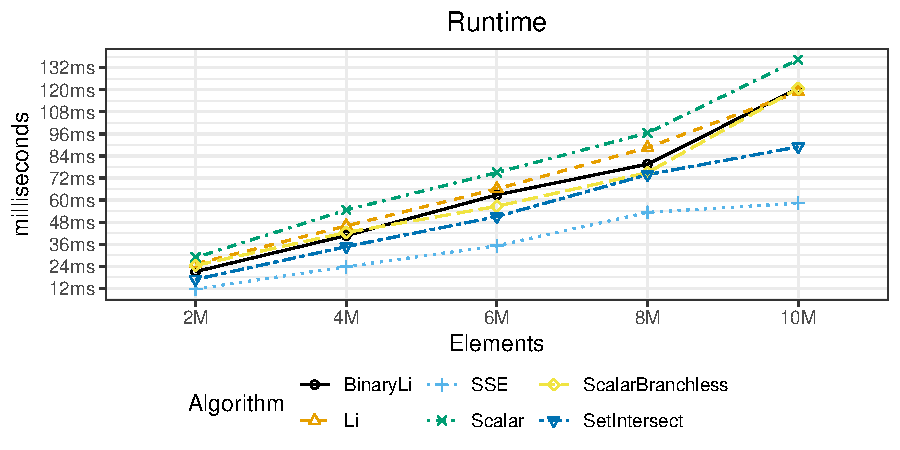
\includegraphics{Figuras/indexResultsPlot-1.pdf}}
  \end{center}
  \vspace{2mm}
  \legenda{Set intersection algorithms response times in milliseconds, ordered by the size of the input relation.}
  \FONTE{Author}
\end{figure}

The SIMD approach is clearly the fastest, however it is also dependant on processor architecture and even though the used SIMD instructions (SS2) are available on almost all modern CPUs, other newer instruction sets might not be, or might have different implementations depending on the CPU vendor, which complicates widespread implementation.

While these tests are interesting, there was not enough time to test some recent benchmarks that found the use of different algorithms and could improve the performance of each, as the use of compressed indexes in \citeonline{pibiriTechniquesInvertedIndex2019} show.
Furthermore, the SIMD instruction set used here (SSE2) is limited even if its support is widespread, with other instruction sets (SSE3, AVX, AVX512, etc) being available on modern CPUs and also available for use.

Some recent results that have not been properly explored in the data cube context as of yet: Recursive Universe Partitioning, a technique that uses the possible search space to partition the sets and execute the intersection~\cite{pibiriFastCompactSet2021}; FESIA, which combines the use of previous techniques with different SIMD computation techniques and a bitmap to decide which algorithm is more suitable for use depending on the set size~\cite{zhangFESIAFastSIMDEfficient2020}, and the use of pre-processed dictionaries to greatly aid in the computation~\cite{dingFastSetIntersection2011a}.
There's even an algorithm to compute the set intersection in $\Theta(1)$ by using a quantum computer and extending from the Bernstein-Vazirani algorithm~\cite{tianQuantumAlgorithmFinding2019}, however due to needing $\mathcal{O}(n)$ quantum storage space, that approach is likely not implementable for any significant dataset in the near future.

Further testing is necessary when dealing with lists of varying sizes, that would showcase the improvements of certain algorithms over others, and the incorporation of these algorithms into a real-world dataset for accurate tests.
Some of the cited documents make decisions of which algorithm to use based on the ratio between the sizes of the two input sets, and this should also be incorporated on future algorithms.

